\minitoc

\pg
We conclude this thesis manuscript with an overview of the results achieved over the course of this doctorate and a discussion of individual items in this larger context. We follow the structure of the manuscript. These conclusions \& discussions are intended to supplement the conclusions \& discussions at the end of each chapter with a synthetic overview of the results of this doctoral thesis.

\pg
The projects undergone as part of this doctoral degree have strong opportunities for future work, both in terms of the algorithmic work \& its application. These will be outlined in detail in the relevant section. It is worth immediately pointing out that only preliminary results were obtained for the application to data by the end of the doctorate's three-year period. These preliminary results are shown in this manuscript, and while they are not of science-grade quality (no astrometric corrections, proper flux bootstrapping, strategy likely needs revisiting for best results) they are nevertheless useful markers of the wealth of information available in the EGS. %, even with the flawed strategy used. Depending on computational resources \& work-hours available, future work could include anything from the creation of a dirty map of the EGS with the data available (which, depending on the runtime for visibility modeling, could be done in time for the defense of this thesis) to a reboot of the strategy, starting explicitly from a model including 3C295 and all other sources at low resolutions (and then improving on 3C295 at high resolutions only). It is a shame that the patchwise imaging of the EGS could not be performed by the end of the thesis, but the author hopes to be able to complete it in due time.



\clearpage

\section{Algorithmic Work}

\pg
One of the aims of this PhD was to develop new interferometric tools \& techniques and to apply them to LOFAR data. This was arguably accomplished successfully:
\begin{itemize}
\item We found a relationship between the statistics of residual visibilities and residual image-plane pixel values (the ``Cov-Cov relationship'').
\item From this relationship, we see that \textbf{calibration artefacts are \textit{directly caused} by correlated calibration gain errors}. In the absence of correlated calibration errors, no artefacts are present.
\item This allowed for a description of the noise-map in the image plane as a constant variance level modulated by a noise-PSF convolved with the sources in the field.
\item This led to the development of an adaptive, quality-based weighting scheme, which reduces the noise in the image (and the presence of calibration artefacts) by minimising either the constant noise term or the noise-PSF.
\item One version of this adaptive, quality-based weighting scheme was successfully applied throughout our data reduction \& wide-field imaging. Other versions are possible, but at the time of writing suffer from issues due to poor conditioning: the development \& deployment of robust versions of these will be the subject of future work.
\end{itemize}

\subsection{The Cov-Cov Relationship}

\pg
The theoretical framework of the cov-cov relationship, which links the variance and covariance in the visibilities to the variance and covariance between pixels in images made with these visibilities, was shown to hold on real data by improving images made with both direction-independent and direction-dependent calibration. This relationship tells us that the variance in images made from interferometric data is the result of two contributions:
\begin{align}
\Cov{\muely} =& \sum_d \Bigg(\sum_b \phi_{bb}^d \left( [\Cov{\matGains}]_{bb} + \frac{w_b^2 \sigma^2}{\phi_{bb}} \right) \muelC_b\nonumber\\
              &+ \sum_{b,b'\ne b}  \phi_{bb'}^d [\Cov{\matGains}]_{bb'} \muelF_{bb'} \Bigg)\label{eq.wever}
\end{align}
which is a repeat of \cref{eq.covcov.matrix}.  
The first term above, which corresponds to the sum over $b$, can be thought of as ``thermal" (i.e. uncorrelated) noise in the visibilities, giving rise to a constant variance throughout the image. The second, which corresponds to sky brightness distribution absorbed into the gain solutions - i.e. correlated noise in the calibration residual visibilities - gives rise to what we call a noise-PSF: a distinctive shape which is convolved with every source in the field (in the case where the true gains are direction-independent), and which gives the distribution function of which calibration artefacts are a single realisation. It corresponds to the sum over $b,b'\ne b$ above - i.e. to those cells of the visibility covariance matrix which are off-diagonal, or correlations between residual visibilities.

\pg
In \cref{eq.wever}, $\Cov{\muely}$ is the covariance matrix of the residual image pixel values, and $\Cov{\matGains}$ is the covariance matrix of the residual visibilities, which is of size $N_b\times N_b$. $[\Cov{\matGains}]_{bb'}$ is a scalar quantity equivalent to the value of the covariance matrix at coordinates $b,b'$. $\phi_{bb'}^d$ corresponds to the product of the weighted\footnote{e.g. Briggs-weighted, quality-weighted, etc} visibilities, associated to a source in direction $d$\footnote{i.e. the visibility which the interferometer would recore if this was the only source in the sky.}, as seen by baselines $b$ and $b'$. $\phi_{bb}^d$ is therefore the square of the magnitude\footnote{i.e. the product of the visibility and its own complex conjugate.} of this quantity for a single baseline and direction. $\sigma^2$ is the thermal noise in the visibilities, which is assumed to be constant for all of them. Finally, $\muelC_b$ is the image-space fringe corresponding to a single baseline, while $\muelF_{bb'}$ is slightly too complex to summarise quickly, but its diagonal maps a single visibility covariance value to a $\deltu\deltv$ fringe, thus determing the artefact distribution around sources in the field.

\pg
Taking the diagonal the matrices shown above gives the ``var-var" relationship, which gives the variance map of the image as a function of the variance in the visibilities. If the visibility covariance matrix is diagonal (i.e. we have no correlated noise in the visibilities), then the second term will be null, and the variance of each pixel in the image-plane will be a constant value (since $\diag{\muelC_b}=\I\forall b$). This is an extremely strong prediction, but one that was validated through simulations: calibration artefacts in interferometric images are due \textit{only} to correlated noise in the visibilities. In the absence of such correlated noise, there will be no calibration artefacts in an image.

\pg
Note that this relationship also confirms, among other things, that ``thermal" noise in interferometric images is actually correlated between pixels, and that this correlation is given exactly by the PSF. This is an expected result, and can only be corrected by fully-deconvolving the PSF from an interferometric image\footnote{Here, when talking about ``fully deconvolving the PSF from an interferometric image", we mean to systematically deconvolve the PSF from each pixel in the image simultaneously. This would be an impractically computationally expensive task, and is therefore not a realistic proposal. Regardless, the point being made here is that the noise of images made using visibilities with purely thermal noise is correlated between pixels - even though the noise is not correlated between visibilities.}. If this is done, then an image made using visibilities containing only uncorrelated noise will itself have noise uncorrelated between pixels, but will not otherwise.

\pg
%
%\pg
%This relationship also confirms, among other things, that ``thermal" noise in interferometric images is actually correlated between pixels, and that this correlation is given exactly by the PSF. This is an expected result, and can only be corrected by fully-deconvolving the PSF from an interferometric image. If this is done, then an image made using visibilities containing only uncorrelated noise will itself have noise uncorrelated between pixels, but will not otherwise.


\subsection{Mapping the variance of images made with interferometric data}

\pg
This relationship was strongly tested through simulations, verifying the noise-PSF behaviour of calibration artefacts in \cref{imag.simu-3sources.noisemap}, reproduced in \cref{whatever}. The visibilities for three point sources were simulated for a single $uv$-track and frequency, and these were multiplied by multiple realisations of time-correlated residual gains. By taking the DFT of each realisation to create dirty maps of this simulated residual map, and calculating the variance for each pixel across our realisations to find the variance map, we see that we do in fact see a PSF-like behaviour in the noise-map, in agreement with our predictions.
\begin{figure}[h!]
\centering
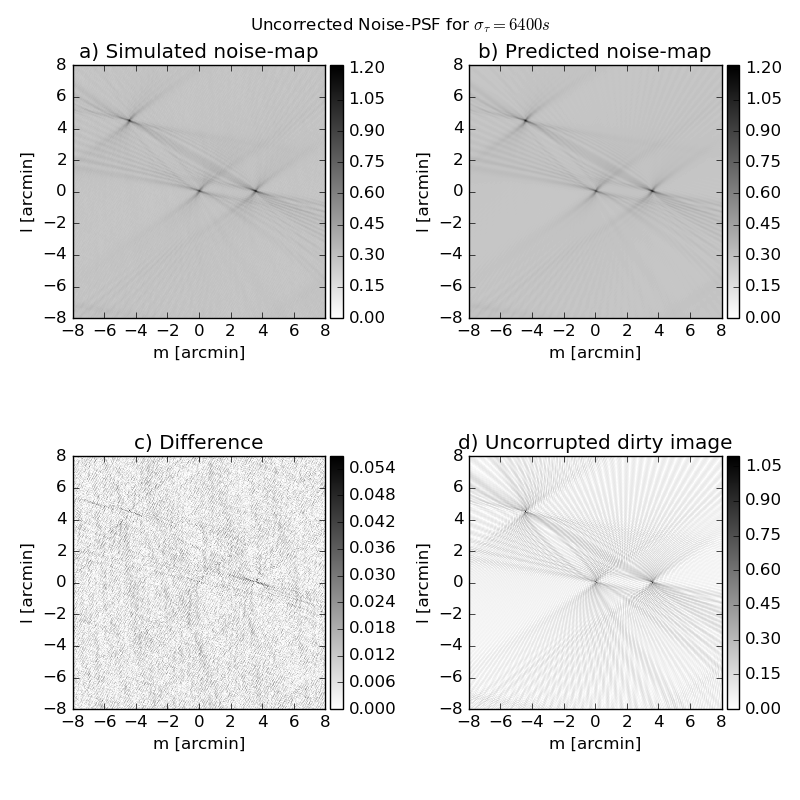
\includegraphics[width=\textwidth]{images/Ctime6400-noisePSFandDirty-uncorr.png}
\caption{\label{whatever} {Noise-map of sky with correlated gain errors and three point sources. The colourbars of (a), (b) and (c) have dimensionless units, while that of (d) is in Jansky. Note the presence of structure in the residuals (c): these show the limits of our hypothesis that sources are well-separated.}}
\end{figure}

\subsection{Quality-based Weighting Schemes}\label{sec.qweights.conclusion}

\pg
The quality-based weighting schemes developed in this section can then be understood as ways to change the noise-distribution: one minimises the constant component of the noise-map, while the other seeks to flatten the noise-PSF. Only the former was implemented for use on real data: the latter suffered from poor conditioning. This weighting scheme consists of down-weighting each visibility by an estimate of the variance of residual.
\begin{align}
w_{b} &= \frac{1}{\Var{\matGains_{b}}}
\end{align}

\begin{figure}[h!]
\begin{subfigure}{.49\textwidth}
\resizebox{\hsize}{!}{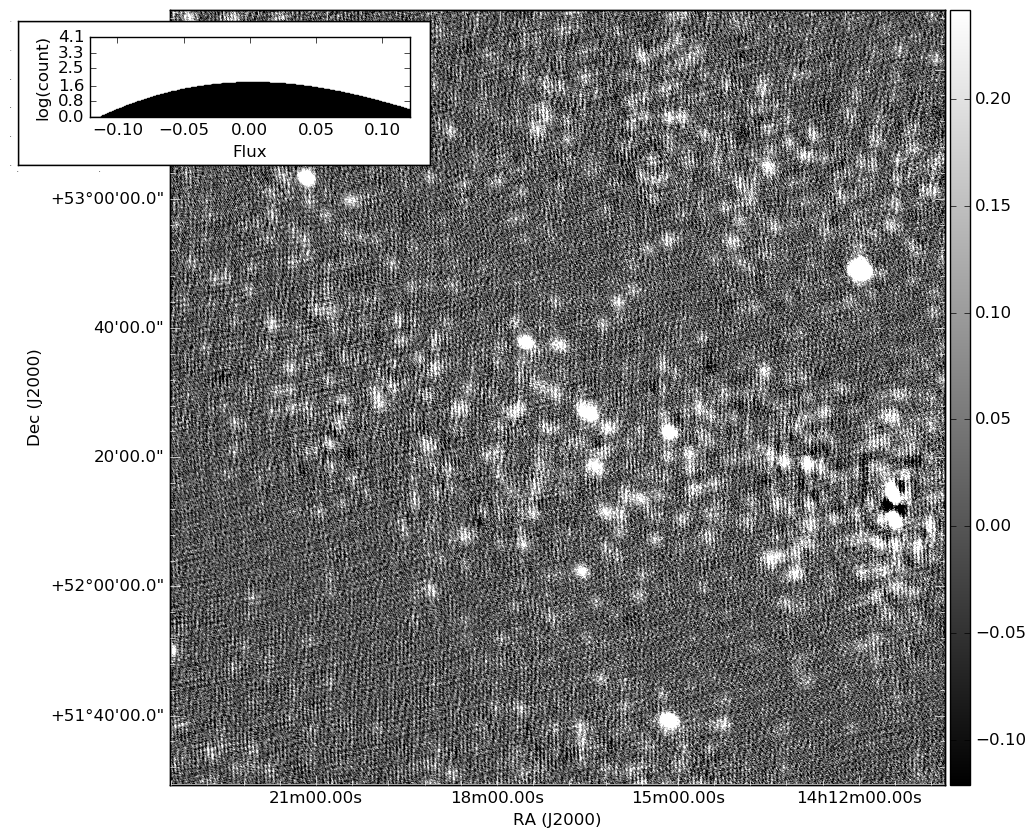
\includegraphics{images/paperfig-noweights.png}}
\caption{\label{image.3c295.nocorr1} Poorly-calibrated, unweighted restored image of the sky near the centre of the Extended Groth Strip. {Units of colourbar are Jy/bm}. rms=86.4mJy/beam}
\end{subfigure}
\begin{subfigure}{.49\textwidth}
\resizebox{\hsize}{!}{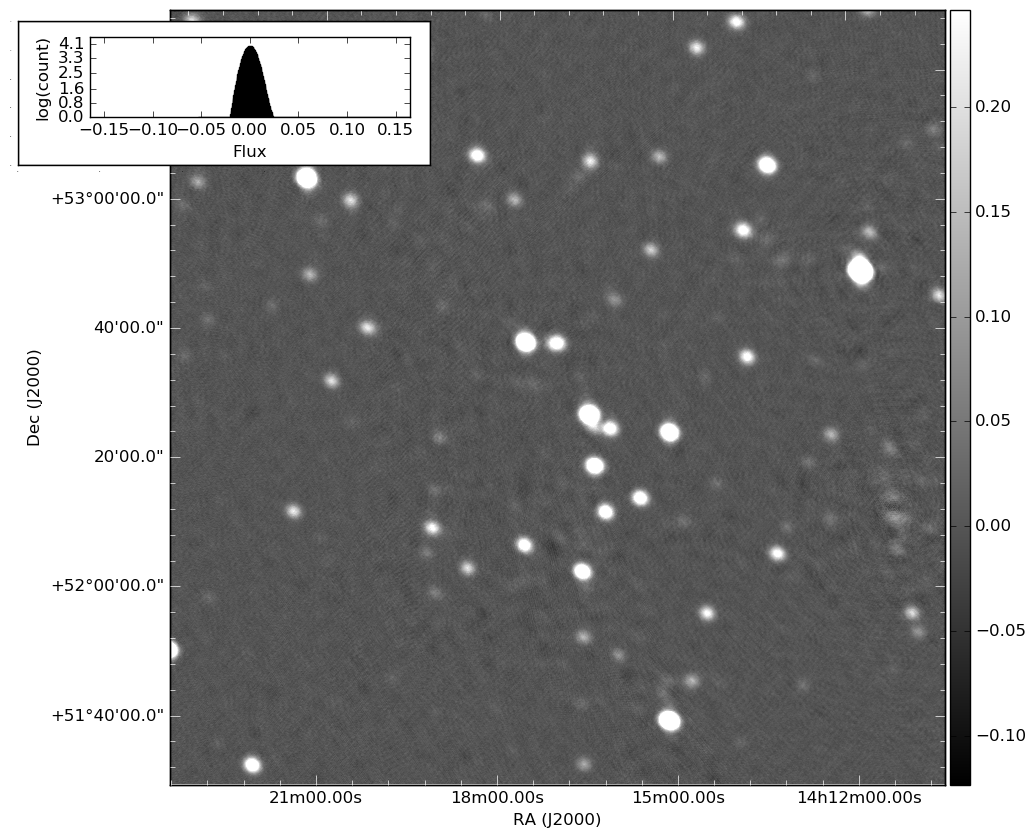
\includegraphics{images/paperfig-antweights.png}}
\caption{\label{image.3c295.antcorr1} Image made with the application of antenna-based, sensitivity-optimal weighting. Solution interval of 2 minutes, half the bandwidth. rms=6.69mJy/beam}
\end{subfigure}
\caption{\label{stuff} Copies of \cref{image.3c295.nocorr} and \cref{image.3c295.antcorr1}, used to show the impact of the weighting schemes on real data.}
\end{figure}

\pg
The cov-cov relationship is likely going to be revisited at a future time to be expanded to more complex cases. Much work nevertheless remains: in both improving the conditioning of the covariance matrix estimation, a necessary prerequisite for its successful application, and in attempting to generalise the framework to account for DDEs, more sophisticated interval solutions (e.g. convolution with a Gaussian with characteristic width equal to the solution interval rather than simple binning), and other modern features of calibration solvers. Similarly, the effect of sky model incompleteness has yet to be investigated thoroughly, and simulation work to this effect could bring great insight on this still-open question.

\pg
Similarly, the question of properly conditioning our estimates of the visibility covariance matrix remains open. This would be a potentially fertile avenue of research, as being able to estimate the full visibility covariance matrix reliably and swiftly could lead to the ability to implement ``artefact-optimal" weights: that is, attempt to completely flatten the noise-PSF, at the cost of increasing the constant, ``thermal" noise component of the image's noise-map.



\section{Imaging the Extended Groth strip}

\pg
We applied our newly-developed weighting schemes to the problem of imaging the Extended Groth Strip, a rich extragalactic field near a bright 3C source. In so doing, we followed a four-part strategy, consisting of:
\begin{itemize}
\item Imaging the full LOFAR primary beam with the core and remote stations. This requires direction-dependent calibration;
\item Creating a high-resolution, frequency-dependent model of 3C295 to use as an international station calibrator source. This required direction-independent self-calibration with a strong imaging $uv$-cut;
\item Preliminary investigation of the impact of directional gain errors from direction-independent calibration using the model of 3C295 obtained from the step above;
\item Creating a high-resolution image of the EGS after subtracting all sources from the widefield image \& the high-resolution model of 3C295.
\end{itemize}

\pg
Of these four points, only the first three were successfully carried out. %Modeling and subtracting all the sources in the primary beam (barring 3C295) proved to be an extremely time-consuming task, and could not be completed in time. 
We therefore limit our discussion to the first three points, treating the last as the subject for future work.

\subsection{Imaging the LOFAR primary beam}

\pg
We begin by creating a decent model of the sky seen by LOFAR's primary beam. To do this, a wide-field, $6''$-resolution image of the fully primary beam was made: this image makes no use of the LOFAR international stations due to technical limitations (memory use). Using PyBDSF \citepads{2015ascl.soft02007M}, this model was extracted from an image made after a few rounds of direction-dependent self-calibration. This direction-dependent self-calibration was done using the killMS/DDF pipeline, which fully models direction-dependent errors due to decorrelation: its application to data is one of the novel contributions of this work.

\pg
This model is still in a very preliminary stage: astrometric errors have not been corrected for, nor has integrated flux bootstrapping been performed. As such, this image (and the model extracted from it) is not of science-grade quality. Even so, and preliminary as it is, it is sensitive and wide-field enough to pick up a good number of interesting diffuse sources. 12 of these were selected to form a so-called ``primary beam galactic zoo" of sources, with the aim of showing the reader the contents of a typical LOFAR deep extragalactic field. They were then matched to NVSS, NVSS \& WISE images to find counterparts: the results are shown in \cref{table.egs.sources1}, which is a repeat of \cref{table.egs.sources}.

\pg
The true interest of modeling these sources at the wide-field resolution achieved is that will allow us to subtract (most of) the emission associated with them when imaging the EGS at high resolution. This, in turns, will allow us to image the EGS itself without pollution from the sidelobes of nearby bright sources. Note that there is nothing inherently special about this field compared to LOTSS fields \citepads{2017A&A...598A.104S}: its interest is in what it can allow us to achieve with the EGS.

%\pg
%Most of the source associations were straightforward, with some of the objects picked out from the wide-field image being well-studied in their own right. Others were not so straightforward, allowing only for individual lobe matching at best. Of course, these results are artisanal in the sense that only a handful of sources were chosen out of over 30000 PyBDSM-identified sources in the field: that these are, by eye, the most interesting in morphological terms does not mean that they are necessarily the most scientifically interesting. Indeed, a proper investigation would require identifying source populations in the LOFAR image after astrometric corrections \& bootstrapping, so as to add a data point in the SEDs of relevant galaxies after matching them with equivalents in other bands. This would represent part of the future work to perform on this dataset, though it would be fruitful to image the full primary beam (and the EGS) using all 40 available hours of observations beforehand, rather than limit ourselves to the 8 used in this doctorate.

\begin{table}[h!]
\begin{tabular}{ccccc}
Name    & RA [hms]    & Dec [dms]   & Likely Association            & LOFAR thumbnail \\\hline
EGS-1   & 14:37:39.53 & 53:36:31.24 & NVSS Radio Galaxy             & \cref{fig.egs1.lofarim} \\
EGS-2   & 14:35:27.84 & 55:07:56.32 & Radio Galaxy in Cluster       & \cref{fig.egs2.lofarim} \\ 
EGS-3   & 14:29:34.13 & 54:43:46.93 & Radio Galaxy in Cluster       & \cref{fig.egs3.lofarim} \\
EGS-4   & 14:31:36.62 & 52:27:33.75 & Radio galaxy, $z=.292$        & \cref{fig.egs4.lofarim} \\
EGS-5   & 14:29:48.89 & 51:10:30.52 & Lobes matched individually    & \cref{fig.egs5.lofarim} \\
EGS-6   & 14:26:04.09 & 51:29:35.07 & One lobe matched individually & \cref{fig.egs6.lofarim} \\
EGS-7   & 14:17:55.58 & 50:08:01.75 & Radio galaxy, $z=.186$        & \cref{fig.egs7.lofarim} \\
EGS-8   & 14:14:40.42 & 51:17:41.00 & Radio galaxy, $z$ unknown     & \cref{fig.egs8.lofarim} \\
EGS-9   & 14:11:36.43 & 52:54:25.53 & Galaxy cluster, $z=.525$      & \cref{fig.egs9.lofarim} \\
EGS-10  & 14:07:09.90 & 55:04:22.23 & Galaxy cluster, $z=.250$      & \cref{fig.egs10.lofarim} \\
EGS-11  & 14:03:16.00 & 51:43:35.23 & Lobes matched individually    & \cref{fig.egs11.lofarim} \\
EGS-12  & 14:02:43.49 & 51:03:14.69 & Radio Galaxy in Cluster       & \cref{fig.egs12.lofarim} \\
\end{tabular}
\caption{\label{table.egs.sources1} Table recapitulating the names, positions and likely associations of all 12 chosen sources in the primary beam. These sources were primarily chosen because they had peculiar or interesting diffuse emission. The associated LOFAR image thumbnails are also given for reference.}
\end{table}

\subsection{Imaging the EGS with LOFAR-VLBI}

\subsubsection{Using 3C295 to self-calibrate the international stations}

\pg
Over the course of this doctoral thesis, I was able to develop an extensive familiarity with the problem of interferometry. Specifically, the work done on self-calibrating 3C295 shows that, while we seem to converge towards the same model regardless of initial conditions (2 point sources, full VLA model, 1 point source\footnote{This initial model was tested, but not followed through to the same extent as the 2-point-source initial model once it became clear that it was both biased away from the ground truth compared to the other two (as we could expect), but that it seemed to converge - albeit very slowly - towards the same ground truth as them.}), this apparent convergence is very slow. As discussed in \cref{sec.CalibImagery}, the problem of imaging is convex (if not necessarily well-conditioned) but the problem of calibration is not fully convex: this introduces the possibility of a net non-convexity in the problem of interferometry. Regardless of whether my experience was that of non-convexity or of poor conditioning leading to impractically slow convergence time, the solution is to regularise.

\pg
One obvious avenue of inquiry likely to yield results would therefore be in the application of amplitude \& phase smoothing on our gain solutions: this corresponds to a regularisation of the calibration inverse problem, improving its conditioning by applying a prior which encourages smooth gain solutions. This prior is physically-motivated, in the sense that we expect the true, underlying gain solutions to be smooth, and so jagged structure in the gains can generally be assimilated to source flux being absorbed into the gain solutions. The tools to perform this smoothing are already developed and being tested on LOTTS DR2 by Cyril Tasse, Tim Shimwell, and Martin Hardcastle. They were not applied here because we used full-Jones calibration solutions (which were found to give better gain solutions with our available SNR early on), whereas the DR2 pipeline solves for scalar gain solutions. Once the smoothing framework is generalised to polarisation, however, its application could result in dramatic improvements in international station gain solutions.


\pg
This work is complementary to that of the LOFAR long-baseline team, and relies heavily on their research \citepads[e.g.]{2016A&A...595A..86J}. In essence, we rely on the fact that 3C295 is a bright, dominant source in the EGS primary beam: assuming that the overall contribution from fainter sources in the field (which peak at $\sim4$Jy, to 3C295's $\sim99$Jy at that frequency) is negligible, then self-calibration on 3C295 ought to yield both an improved model of that source \textbf{and} good gain solutions for the international LOFAR stations. One point of originality of this work is that we consistently take into account direction-dependent errors due to decorrelation (but not DDEs) - this has only become possible recently, with the appropriate modeling of decorrelation both in imaging (through the direction-dependent PSF) \textit{and} calibration (by modeling the decorrelation of model sources properly when creating model visibilities). This removes one of the sources of bias in solving the overlal problem of interferometry, and allows calibrator sources outside phase centre to be used reliably.

\pg
As it turns out, this was a bold assumption to make: the model resulting from our self-calibration is still rife with calibration artefacts. Based on our understanding of the cov-cov relationship, many of these can be understood as being due to sky brightness being absorbed into the gain solutions: gain inspection supports this theory, showing unexpected and correlated structure in our international station gain amplitude solutions. 

\pg
Other avenues remain open to go beyond this issue: using the full low-resolution primary beam sky model from \cref{section.EGS.lowres} could be one way to improve our images. However, we would still find ourselves with much unmodeled emission on the baselines including an international station. Another possible avenue of improvement would be through the use the EHT-imager tools: these rely on fitting model data to closure quantities (amplitude \& phase), which are unaffected by antenna-based errors. This is currently being tested by the long baseline working group.

\pg
All these avenues of research are, of course, only possible because we find ourselves in very specific circumstances: the presence of a very bright resolved source in a famous (and therefore relatively well-known) extragalactic field. As such, we have the freedom to explore methods which supplement those of the LBCS team, who are more strongly constrained in that their aim is to provide a solid, reliable catalog of sources suitable for calibrating the international LOFAR stations. This, in turns, requires a solid, reliable strategy, in ways that our relatively straightforward application to a single field does not.

\subsubsection{Quantifying the impact of international station directional gain errors}

\pg
This work is strongly linked to the self-calibration on 3C295: depending on the quality of both the model and the gain solutions attained (i.e. of how the quality of our solution to the overall inverse problem of radio interferometry), directional gain errors will be more or less present across the primary beam.

\pg
We choose 8 nearby sources from the LBCS, a catalogue of compact radio sources in the Northern sky, spread around both the EGS and 3C295. These are reprinted below, in copies of \cref{table.LOBOS.sources} and \cref{lbcs-coverage-image}. Two direction-dependent effects are expected to arise, one as a function of distance from phase centre (i.e. from the EGS) and the other as a function of distance from the direction-independent calibration source (i.e. from 3C295). %These distances are summarised  in \cref{table.LOBOS.sources1} and \cref{lbcs-coverage-image1} below.


\pg
The direction-dependent effect which is function of distance from the EGS, decorrelation, is modeled in the DDF/kMS pipeline. As such, we do not expect this effect to dominate. The other direction-dependent effect, function of distance from 3C295, however, is not modeled: this effect corresponds to directional gain errors. Direction-independent calibration is only exact in the direction of the calibrator source when a single source is present in the field of view; this is because, in reality, the astrophysical signal from each source in the field of view reaches us through a slightly different ionosphere, are in areas of the antenna beam which are 
of varying sensitivity, etc. Some of these models can be modeled and corrected to some degree (e.g. LOFAR beam), while others cannot at the time of writing (ionospheric effects). 
%
%\begin{table}[h!]
%\begin{tabular}{ccccc}
%\# & RA [hms]    & Dec [dms]   & Dist. from EGS [deg.] & Dist. from 3C295 [deg.] \\\hline
%1  & 14:30:18.72 & 52:17:29.80 & 2.041                         & 2.904 \\
%2  & 14:19:44.44 & 54:23:04.58 & 1.928                         & 2.517 \\ 
%3  & 14:21:20.05 & 53:03:46.00 & 0.864                         & 1.743 \\
%4  & 14:21:09.41 & 51:22:32.46 & 1.294                         & 1.728 \\
%5  & 14:11:50.32 & 52:49:02.66 & 0.844                         & 0.619 \\
%6  & 14:11:20.23 & 52:12:04.30 & 0.915                         & 0.000 \\
%7  & 14:08:07.00 & 52:55:11.36 & 1.409                         & 0.869 \\
%8  & 14:08:09.76 & 52:44:46.56 & 1.354                         & 0.680 \\
%\end{tabular}
%\caption{\label{table.LOBOS.sources1}Table giving the positions of our 8 LBCS sources and their distance from both the centre of the EGS and 3C295.}
%\end{table}
%\begin{figure}[h!]
%\includegraphics[width=.93\linewidth]{images/{image_full_ampphase_di_m.NS_Smooth.noise01.fitslbcs.egs.positions}.png}
%\caption{Position of the calibrator sources around the EGS, overlaid on the widefield EGS image. LBCS is 3C295.}
%\label{lbcs-coverage-image1}
%\end{figure}

\pg
With our final model of 3C295 and gain solutions, flawed as they are, we find that there is little direction-dependent variation in calibration artefact intensity for the various LBCS sources in the field. This is a strong encouragement to continue the project and move on to imaging the EGS using international LOFAR stations.

\subsection{Future Work}

\pg
As mentioned in \cref{sec.qweights.conclusion}, there is much work ahead of us with regards to the algorithmic work developed in this doctoral thesis. Not only can the theoretical framework be expanded to include more complex cases, but those results which it already provides are limited by the conditioning of our estimation of the visibility covariance matrix. There is therefore room for both expanding on and improving existing results.

\pg
As for the application to data, it is very encouraging to see that not only are multiple LBCS sources resolved to show physically-sensible morphologies (FRI, FRII, headtail radio galaxies, etc), but in some instances are even resolved to show not just one, but multiple sources with physically-sensible morphology. Many of the LBCS candidates appear to be double or even triple sources. This would indicate that the directional gain errors for many of the LBCS sources are not so strong that they deteriorate the image beyond the recovery of such morphological information; since calibration artifacts, DDEs included, are more present near bright sources, the fact that they are not strong enough to pollute LBCS sources is a promising indicator that even fainter sources in the EGS have recoverable morphological information, given our data and calibration strategy.

\pg
However, we were not able to create images of this field before the end of this doctoral degree: creating this image (and performing the associated quality-control and source extraction) is therefore very high indeed on the priority for future work. The preliminary results shown in this manuscript are not of science-grade quality (no astrometric corrections, proper flux bootstrapping, strategy likely needs revisiting for best results), but they are nevertheless useful markers of the wealth of information available in the EGS as seen with the full LOFAR array. %, even with the flaws in our strategy. 


%
%\pg
%For the second item, a high-resolution, frequency-dependent model of 3C295 was successfully obtained. With this model, the international LOFAR stations were calibrated well enough that other calibrator sources were visible and morphologically-interesting, even with strong Briggs weighting (optimising for resolution at the cost of signal-to-noise). Other sources in the field were visible; with the proper subtraction of 3C295 and the other sources in the field, a dirty map of the EGS would be within easy reach, and all that remains would be to deconvolve it. This is a relatively straightforward but time-consuming operation. Afterwards, the necessary checks (integrated flux, source completeness, astrometric accuracy) will need to be performed before the image is scientifically useful. 
%
%
%\pg
%Much work thus remains. Due to a series of setbacks and complications, only very preliminary results were obtained by the end of the doctorate's three-year period. These preliminary results are shown in this manuscript, and while they are not of science-grade quality (no astrometric corrections, proper flux bootstrapping, strategy likely needs revisiting for best results) they are nevertheless useful markers of the wealth of information available in the EGS, even with the flawed strategy used. Depending on computational resources \& work-hours available, future work could include anything from the creation of a dirty map of the EGS with the data available (which, depending on the runtime for visibility modeling, could be done in time for the defense of this thesis) to a reboot of the strategy, starting explicitly from a model including 3C295 and all other sources at low resolutions (and then improving on 3C295 at high resolutions only). It is a shame that the patchwise imaging of the EGS could not be performed by the end of the thesis, but the author hopes to be able to complete it in due time.

%
%\pg
%The algorithmic work done in this PhD was extremely fruitful, though its applications to data were less so. Much future work remains: in particular, imaging the EGS has not yet been done, due to technical \& time constraints (1 day / subband to model visibilities for out-of-field source subtraction). 